\section{סקירת ספרות}

השימוש במודלים מבוססי נתונים \LR{(Data-Driven Models)} בחקלאות מדייקת צבר תאוצה בשנים האחרונות, ומאפשר להחליף מדידות פיזיקליות יקרות באמצעות אלגוריתמים המעבדים נתוני סביבה ותפעול. עם זאת, יישום מודלים אלו במערכות דינמיות כמו חממות מחייב התמודדות עם אירועי קצה חריגים כגון קפיצות מליחות או צניחת pH. אתגר זה דורש מהמודל לא רק לחזות בדיוק מצבי שגרה מוכרים (אינטרפולציה), אלא גם לבצע אקסטרפולציה אמינה מחוץ לטווח הנתונים ההיסטורי.

כדי להתמודד עם אתגר זה, סקירה זו משלבת שני צירי ספרות: הראשון בוחן יישומי למידה עמוקה לחיזוי משתני קרקע בחקלאות, והשני מתמקד בספרות האלגוריתמית הבוחנת את מגבלות עצי ההחלטה, ומבססת את הצורך בארכיטקטורה היברידית המשלבת רכיב ליניארי למצבי קיצון.

אחד האתגרים המרכזיים בגידול בחממות הוא השליטה ברמת המליחות (EC) בבית השורשים. במחקרם של \LR{Moon et al.\ (2018)} בחנו החוקרים את היכולת לחזות את ה-EC של תמיסת ההזנה במערכות הידרופוניות סגורות \LR{(Closed-loop soilless cultures)}. החוקרים השתמשו ברשת נוירונים מסוג RNN \LR{(Recurrent Neural Network)} ובפרט במודל LSTM הידוע ביכולתו ללמוד סדרות עיתיות. המחקר הראה כי שילוב של משתני אקלים (קרינה, טמפרטורה ולחות יחסית) יחד עם נתוני תפעול (כמות השקיה וריכוז דשן במי ההשקיה), מאפשר לחזות בדיוק רב את ה-EC העתידי במצע. המסקנה המרכזית ממחקר זה, הרלוונטית לעבודתנו, היא שקיים קשר הדוק וניתן למידול בין עומס האקלים החיצוני לבין הדינמיקה הכימית בבית השורשים, וכי היסטוריית הנתונים \LR{(Time-lagged features)} היא קריטית לביצועי המודל.

בעוד ש-Moon התמקד בכימיה של המים, \LR{Lü et al.\ (2025)} הציגו גישה מתקדמת לחיזוי רטיבות קרקע בבית השורשים \LR{(RZSM -- Root Zone Soil Moisture)}. המחקר התמודד עם הקושי למדוד רטיבות בעומק הקרקע והציע מודל היברידי המשלב מודל פיזיקלי הידרולוגי (Hydrus-1D) עם מודל למידה עמוקה מסוג CNN-LSTM-Attention. המחקר הדגים כיצד מודלים של למידה עמוקה \LR{(Deep Learning)} יכולים ללמוד את הקשרים הלא-ליניאריים המורכבים בין רטיבות פני השטח (הניתנת למדידה קלה או חישה מרחוק) לבין המתרחש בעומק בית השורשים. השימוש במנגנון קשב \LR{(Attention Mechanism)} אפשר למודל להתמקד בטווחי הזמן המשפיעים ביותר על המצב הנוכחי. אף על פי שמחקר זה בוצע בתנאי שדה \LR{(Oasis field)} ולא בחממה, הוא מחזק את ההנחה כי ניתן לייצר "חיישן וירטואלי" לתנאי עומק הקרקע על בסיס נתונים סביבתיים, וכי שילוב של ארכיטקטורות המביאות בחשבון את המימד הרציף של הזמן כגון LSTM או נגזרותיו משפר משמעותית את הדיוק בהשוואה למודלים סטטיים.

לצד היתרונות של מודלים אלו במצבי שגרה, הציר השני בספרות מתמקד בבחירת ארכיטקטורת האלגוריתם המתאימה להתמודדות עם חריגות מהדפוסים המוכרים. במחקרם של \LR{Muckley et al.\ (2023)} נבחנה שאלת האקסטרפולציה במודלים מדעיים מבוססי למידת מכונה. החוקרים השוו בין מודלים מורכבים מסוג \LR{Random Forest} ורשתות נוירונים לבין מודלים ליניאריים פשוטים, תוך התמקדות בבעיות מתחום מדעי החומרים. ממצאי המחקר הראו כי מודלים מורכבים נוטים להציג ביצועים טובים יותר במצבי אינטרפולציה, שבהם הדוגמאות החדשות נמצאות בתוך תחום הנתונים שנלמד. לעומת זאת, כאשר נדרשה אקסטרפולציה מעבר לטווח הנתונים, המודלים הליניאריים הפשוטים היו תחרותיים מאוד ולעיתים אף הציגו ביצועים טובים יותר -- ממצא התומך בשילוב רכיב ליניארי במצבים שבהם המערכת חורגת מהדפוסים הרגילים.

לעומת זאת, במחקרם של \LR{Loh et al.\ (2007)} הוצגה תמונה זהירה וממוקדת יותר לגבי אקסטרפולציה בסביבת עצים. החוקרים בחנו עצי מודל ליניאריים \LR{(Linear Model Trees)}, כלומר עצים שבהם בכל עלה מותאם מודל ליניארי מקומי, והראו כי אף על פי שמבנה כזה מאפשר למודל להמשיך מגמות מעבר לטווח הנתונים, הוא עלול גם ליצור שגיאות גדולות (קטסטרופליות) כאשר ההנחה הליניארית מופעלת רחוק מדי ממרכז הנתונים בעלה הספציפי. ממצא זה מדגיש כי רכיב ליניארי אינו צריך להחליף את המודל המרכזי, אלא לפעול בזהירות, באופן מוגבל ומבוקר, ומצדיק שימוש במודלים משלימים רובסטיים כגון רגרסיית הובר \LR{(Huber Regressor)} הניחנת בעמידות גבוהה בפני תצפיות חריגות (Outliers).

גישה המחזקת תפיסה היברידית זו מופיעה במחקרם של \LR{Friedberg et al.\ (2021)}, שבו הוצע לשלב בין \LR{Random Forest} לבין התאמה ליניארית מקומית \LR{(Local Linear Forests)}. החוקרים ציינו כי יערות אקראיים הם מודלים חזקים וגמישים ללמידת קשרים לא-ליניאריים, אך יש להם מגבלה מובנית בתיאור אותות חלקים ומגמות רציפות \LR{(Continuous trends)}. כדי להתמודד עם מגבלה זו, הם שילבו את מנגנון החלוקה של היער עם רגרסיה ליניארית מקומית, כך שהמודל שומר על היתרון של עצים בזיהוי אזורים ודפוסים, אך מוסיף יכולת טובה יותר לתיאור מגמות רציפות. באופן דומה, במחקרם של \LR{Cai et al.\ (2023)} הוצע מודל בשם \LR{Extrapolated Random Tree for Regression} שמטרתו לשפר את יכולת האקסטרפולציה של עצי רגרסיה באמצעות שילוב מנגנון אקסטרפולציה המבוסס על רגרסיה ליניארית בתוך מבנה העץ, ובכך הוכח כי שילוב רכיב אקסטרפולטיבי משפר משמעותית את ביצועי המודל מחוץ לטווח המוכר.

הספרות הקיימת מצביעה על היתכנות גבוהה לשימוש בלמידת מכונה לניטור בית השורשים. בעוד ש-Moon et al.\ התמקדו ב-EC ו-Lü et al.\ ברטיבות, פרויקט זה שואף לשלב גישות אלו ולפתח מודל אחוד החוזה הן את ה-EC והן את ה-pH, תוך שימוש באלגוריתמים של למידת מכונה מבוססי עצים המציעים איזון בין דיוק ליכולת פרשנות ומתאימים ליישום במערכות בקרה תפעוליות בחממות מסחריות. יחד עם זאת, לאור מגבלות האקסטרפולציה של מודלים מורכבים במצבי קצה, כפי שעולה ממחקריהם של Muckley, Loh, Friedberg ו-Cai, הפרויקט אינו נשען על אלגוריתם בודד. תחת זאת, מיושמת גישה היברידית: שימוש באלגוריתמים מבוססי-עצים המציעים איזון בין דיוק ליכולת פרשנות במצבי שגרה, בשילוב רכיב ליניארי מבוקר המבטיח יציבות באירועים חריגים. שילוב זה מייצר מודל שלם ואמין, המותאם ליישום מעשי במערכות בקרה תפעוליות בחממות מסחריות.

\begin{figure}[H]
    \centering
    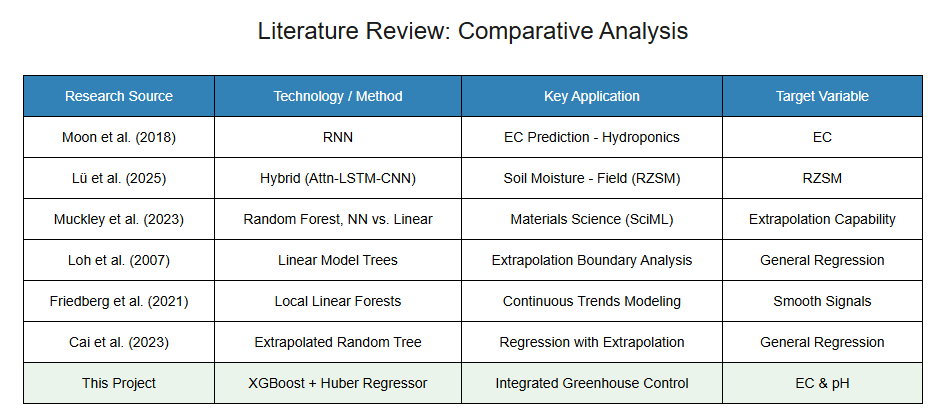
\includegraphics[width=\textwidth]{figures/fig03.png}
    \caption{\LR{Literature Review -- Comparative Analysis of Related Methods}}
    \label{fig:litreview}
\end{figure}

איור \ref{fig:litreview} מסכם את המחקרים שנסקרו, את השיטות שבהן נעשה שימוש, את יישומם המרכזי ואת המשתנה החזוי, לצד מיקומו של פרויקט זה במרחב זה.
